\documentclass[10pt]{article}
\usepackage[letterpaper]{geometry}
\geometry{verbose,tmargin=1in,bmargin=1in,lmargin=1in,rmargin=1in}
\usepackage{setspace}
\usepackage{ragged2e}
\usepackage{color}
\usepackage{titlesec}
\usepackage{graphicx}
\usepackage{float}
\usepackage{mathtools}
\usepackage{amsmath}
\usepackage[font=small,labelfont=bf,labelsep=period]{caption}
\usepackage[english]{babel}
\usepackage{indentfirst}
\usepackage{array}
\usepackage{makecell}
\usepackage[usenames,dvipsnames]{xcolor}
\usepackage{multirow}
\usepackage{tabularx}
\usepackage{arydshln}
\usepackage{caption}
\usepackage{subcaption}
\usepackage{xfrac}
\usepackage{etoolbox}
\usepackage{cite}
\usepackage{url}
\usepackage{dcolumn}
\usepackage{hyperref}
\usepackage{courier}
\usepackage{url}
\usepackage{esvect}
\usepackage{commath}
\usepackage{verbatim} % for block comments
\usepackage{enumitem}
\usepackage{hyperref} % for clickable table of contents
\usepackage{braket}
\usepackage{titlesec}
\usepackage{booktabs}
\usepackage{gensymb}
\usepackage{longtable}
\usepackage{listings}
\usepackage{cancel}
\usepackage{tcolorbox}
\usepackage[mathscr]{euscript}
\lstset{
    frame=single,
    breaklines=true,
    postbreak=\raisebox{0ex}[0ex][0ex]{\ensuremath{\color{red}\hookrightarrow\space}}
}

% for circled numbers
\usepackage{tikz}
\newcommand*\circled[1]{\tikz[baseline=(char.base)]{
            \node[shape=circle,draw,inner sep=2pt] (char) {#1};}}


\titleclass{\subsubsubsection}{straight}[\subsection]

% define new command for triple sub sections
\newcounter{subsubsubsection}[subsubsection]
\renewcommand\thesubsubsubsection{\thesubsubsection.\arabic{subsubsubsection}}
\renewcommand\theparagraph{\thesubsubsubsection.\arabic{paragraph}} % optional; useful if paragraphs are to be numbered

\titleformat{\subsubsubsection}
  {\normalfont\normalsize\bfseries}{\thesubsubsubsection}{1em}{}
\titlespacing*{\subsubsubsection}
{0pt}{3.25ex plus 1ex minus .2ex}{1.5ex plus .2ex}

\makeatletter
\renewcommand\paragraph{\@startsection{paragraph}{5}{\z@}%
  {3.25ex \@plus1ex \@minus.2ex}%
  {-1em}%
  {\normalfont\normalsize\bfseries}}
\renewcommand\subparagraph{\@startsection{subparagraph}{6}{\parindent}%
  {3.25ex \@plus1ex \@minus .2ex}%
  {-1em}%
  {\normalfont\normalsize\bfseries}}
\def\toclevel@subsubsubsection{4}
\def\toclevel@paragraph{5}
\def\toclevel@paragraph{6}
\def\l@subsubsubsection{\@dottedtocline{4}{7em}{4em}}
\def\l@paragraph{\@dottedtocline{5}{10em}{5em}}
\def\l@subparagraph{\@dottedtocline{6}{14em}{6em}}
\makeatother

\newcommand{\volume}{\mathop{\ooalign{\hfil$V$\hfil\cr\kern0.08em--\hfil\cr}}\nolimits}

\setcounter{secnumdepth}{4}
\setcounter{tocdepth}{4}
\begin{document}

\title{ME 280a: HW 6}
\author{April Novak}

\maketitle

\section{Introduction and Objectives}

The purpose of this study is to construct the Finite Element (FE) problem statement for a 2-D heat conduction problem, and then to solve said problem on a relatively complex domain.

\section{Procedure}
\label{sec:Procedure}

This section details the problem statement and mathematical method used for solving the problem.

\subsection{The Analytical Solution}

This problem solves the heat conduction problem, with a governing equation given by:

\begin{equation}
\nabla\cdot(k\nabla T)+f=0
\end{equation}

where \(k\) is the thermal conductivity, \(T\) the temperature (scalar), and \(f\) a volumetric heat source/sink. This problem is to be solved with two different sets of specifications. For one of these sets, there is an analytical solution to offer a comparison to ensure that the code functions correctly, and for the second, there is no analytical solution. Both specifications have the following boundary conditions:

\begin{equation}
\begin{aligned}
T(\theta=\pi)=T_0\\
-k\nabla T\cdot\hat{n}|_{\theta=0}=q_o(r)\\
-k\nabla T\cdot\hat{n}|_{\theta\neq0\cup \theta\neq\pi}=0\\
\end{aligned}
\end{equation}

For the analytical solution, these specifications are:

\begin{equation}
\label{eq:AnalyticalSpecs}
\begin{aligned}
T_o=110\\
q_o(r)=\frac{20}{r}\\
f(r,\theta)=\frac{40}{r^2}\sin{(2\theta)}\\
\end{aligned}
\end{equation}

To obtain the analytical solution, the governing equation is written explicitly in polar coordinates:

\begin{equation}
\frac{1}{r}\frac{\partial}{\partial r}\left(kr\frac{\partial T}{\partial r}\right)+\frac{1}{r^2}\frac{\partial}{\partial\theta}\left(k\frac{\partial T}{\partial\theta}\right)+\frac{40}{r^2}\sin{(2\theta)}=0
\end{equation}

where \(f(r,\theta)\) has been inserted from Eq. \eqref{eq:AnalyticalSpecs}. Because \(k\) is constant with these specifications, it can be moved outside the derivatives. Because boundary conditions are only asymmetric in the \(\theta\) direction (i.e. boundary conditions are insulated on the \(r\)-sides of the tube), the solution is not a function of \(r\). 

\begin{equation}
k\frac{\partial}{\partial\theta}\left(\frac{\partial T}{\partial\theta}\right)+40\sin{(2\theta)}=0
\end{equation}

Rearranging, and integrating once in \(\theta\):

\begin{equation}
d\left(\frac{d T}{d\theta}\right)=-\frac{40}{k}\sin{(2\theta)}d\theta\quad\rightarrow\quad \frac{dT}{d\theta}=\frac{20}{k}\cos{(2\theta)}+C_o
\end{equation}

Integrating once more:

\begin{equation}
T(\theta)=\frac{10}{k}\sin{(2\theta)}+C_o\theta+C_1
\end{equation}

where \(C_o\) and \(C_1\) are constants of integration. These constants are determined by applying the boundary conditions:

\begin{equation}
T(\pi)=T_o=C_o\pi+C_1
\end{equation}

\begin{equation}
-k\frac{1}{r}\frac{dT(\theta=0)}{d\theta}=-k\frac{1}{r}\left(\frac{20}{k}+C_o\right)=\frac{20}{r}
\end{equation}

These equations give:

\begin{equation}
\begin{aligned}
C_1=T_o-\frac{40}{k}\pi\\
C_o=\frac{40}{k}\\
\end{aligned}
\end{equation}

\subsection{The Weak Form}

The weak form is obtained by multiplying through by a test function \(\psi\) and integrating over the body:

\begin{equation}
\label{eq:StrongForm2}
\int_{\Omega}\nabla\cdot(k\nabla T)\psi d\Omega=-\int_{\Omega}f\psi d\Omega
\end{equation}

Applying the product rule in Eq. \eqref{eq:StrongForm2}:

\begin{equation}
\begin{aligned}
-\int_{\Omega}k\nabla T\nabla\psi d\Omega+\int_{\partial\Omega}k\nabla T\psi\cdot\hat{n}dA=-\int_{\Omega}f\psi d\Omega\\
\int_{\Omega}k\nabla T\nabla\psi d\Omega=\int_{\Omega}f\psi d\Omega+\int_{\partial\Omega}k\nabla T\psi\cdot\hat{n}dA\\
\end{aligned}
\end{equation}

Because the shape functions are defined to be zero on Dirichlet boundaries, the above area integral can be specified as the boundaries over which there are flux boundary conditions:

\begin{equation}
\int_{\Omega}k\nabla T\nabla\psi d\Omega=\int_{\Omega}f\psi d\Omega+\int_{\Gamma_q}\textbf{q}^{*}\psi dA\\
\end{equation}

where \(\Gamma_q\) is the boundary over which the heat flux is specified, and \(\textbf{q}^{*}=k\nabla T\cdot\hat{n}\) is the known heat flux on the boundary. On boundaries for which there are Dirichlet conditions, denoted as \(\Gamma_d\), those nodes are either subject to a penalty term to enforce the boundary, or those nodes are removed from the final matrix system. Both of these methods are investigated in this assignment - the method of removing nodes from the global stiffness matrix and load vector will be referred to as ``static condensation.'' Hence, the weak form can be stated as:

\begin{tcolorbox}
\begin{equation}
\label{eq:WeakFormQ1}
\begin{aligned}
\text{Find }T\in \textbf{H}^T(\Omega)\subset \textbf{H}^1(\Omega) \text{ so that } T|_{\Gamma_d}=T^{*} \text{ and so that }\forall\ \psi \in \textbf{H}^\psi(\Omega)\subset \textbf{H}^1(\Omega), \psi|_{\Gamma_d}=\textbf{0},\\
\text{and for }\textbf{q}\in\textbf{L}^2(\Gamma_q), \textbf{q}=\textbf{q}^{*}|_{\Gamma_q}\text{ and }f\in\textbf{L}^2(\Omega)\\
\int_{\Omega}k\nabla T\nabla\psi d\Omega=\int_{\Omega}f\psi d\Omega+\int_{\Gamma_q}\textbf{q}^{*}\psi dA\\
\end{aligned}
\end{equation}
\end{tcolorbox}

where this weak form applies if the method of static condensation is to be used to apply the Dirichlet boundary conditions. If the penalty method is to be used:

\begin{tcolorbox}
\begin{equation}
\label{eq:WeakFormQ2}
\begin{aligned}
\text{Find }T\in \textbf{H}^T(\Omega)\subset \textbf{H}^1(\Omega) \text{ so that } T|_{\Gamma_d}=T^{*} \text{ and so that }\forall\ \psi \in \textbf{H}^\psi(\Omega)\subset \textbf{H}^1(\Omega)\\
\text{and for }\textbf{q}\in\textbf{L}^2(\Gamma_q), \textbf{q}=\textbf{q}^{*}|_{\Gamma_q}\text{ and }f\in\textbf{L}^2(\Omega)\\
\int_{\Omega}k\nabla T\nabla\psi d\Omega+P^{*}\int_{\Gamma_d}T\psi dA=\int_{\Omega}f\psi d\Omega+\int_{\Gamma_q}\textbf{q}^{*}\psi dA+P^{*}\int_{\Gamma_d}T^{*}\psi dA\\
\end{aligned}
\end{equation}
\end{tcolorbox}

where \(P^{*}\) is the penalty coefficient that is a large, positive number that essentially applies a traction that forces the temperature on the Dirichlet boundaries to equal the specified temperature \(T^{*}\). 

\subsubsection{The Finite Element Weak Form}

This section covers the details regarding finite element implementation of Eq. \eqref{eq:WeakFormQ2} (the non-penalty method simply sets \(P^{*}=0\). To implement this weak form, first the unknown, the temperature, must be expanded in a series of shape functions \(\phi\):

\begin{equation}
T=\sum_{i=1}^{n_{en}}C_j\phi_j=\textbf{N}\textbf{T}
\end{equation}

where \(n_{en}\) are the number of nodes per element and the following vectors have been defined (for a linear, 2-D element):

\begin{equation}
\textbf{N}\equiv\begin{bmatrix}\phi_1(x,y) & \phi_2(x,y) & \phi_3(x,y) & \phi_4(x,y)
\end{bmatrix}
\end{equation}

\begin{equation}
\textbf{T}\equiv\begin{bmatrix}C_1 &  C_2 & C_3 & C_4
\end{bmatrix}^T
\end{equation}

Likewise, the weight function is also expanded in a series of these shape functions. The gradient of temperature is required in the weak form:

\begin{equation}
\nabla T=\frac{\partial T}{\partial x}\hat{x}+\frac{\partial T}{\partial y}\hat{y}=\textbf{B}\textbf{T}
\end{equation}

where the following matrix is defined:

\begin{equation}
\textbf{B}\equiv\begin{bmatrix}\frac{\partial \phi_1}{\partial x} & \frac{\partial \phi_2}{\partial x} & \frac{\partial \phi_3}{\partial x} & \frac{\partial \phi_4}{\partial x}\\
\frac{\partial \phi_1}{\partial y} & \frac{\partial \phi_2}{\partial y} & \frac{\partial \phi_3}{\partial y} & \frac{\partial \phi_4}{\partial y}\\
\end{bmatrix}
\end{equation}

The weak form can now be written using these definitions:

\begin{equation}
\label{eq:WeakFormQ3}
\begin{aligned}
\int_{\Omega}k\textbf{B}\textbf{T}\cdot(\textbf{B}\Psi) d\Omega+P^{*}\int_{\Gamma_d}\textbf{N}\textbf{T}\cdot(\textbf{N}\Psi)dA=\int_{\Omega}f\textbf{N}\Psi d\Omega+\int_{\Gamma_q}\textbf{q}^{*}(\textbf{N}\Psi) dA+P^{*}\int_{\Gamma_d}T^{*}(\textbf{N}\Psi) dA\\
\end{aligned}
\end{equation}

Then, noting that the dot product of two vectors can be written as \(\textbf{a}\cdot\textbf{b}=\textbf{b}^T\textbf{a}\), and noting the equivalence between \(\textbf{N}\Psi\) and \((\textbf{N}\Psi)^T\):

\begin{equation}
\int_{\Omega}(\textbf{B}\Psi)^Tk\textbf{B}\textbf{T} d\Omega+P^{*}\int_{\Gamma_d}(\textbf{N}\Psi)^T\textbf{N}\textbf{T}dA=\int_{\Omega}f(\textbf{N}\Psi)^T d\Omega+\int_{\Gamma_q}\textbf{q}^{*}(\textbf{N}\Psi)^T dA+P^{*}\int_{\Gamma_d}T^{*}(\textbf{N}\Psi)^T dA\\
\end{equation}

The transpose of a product is:

\begin{equation}
(AB)^T=A^TB^T
\end{equation}

Using this identity, \(\Psi^T\) cancels from every term (to be more exact, the above could be rearranged such that \(\Psi\) multiplies every term within an integrand, and that term equals zero, in which case the term multiplied by \(\Psi\) must also be zero). 

\begin{equation}
\int_{\Omega}\textbf{B}^Tk\textbf{B}\textbf{T} d\Omega+P^{*}\int_{\Gamma_d}\textbf{N}^T\textbf{N}\textbf{T}dA=\int_{\Omega}f\textbf{N}^T d\Omega+\int_{\Gamma_q}\textbf{q}^{*}\textbf{N}^T dA+P^{*}\int_{\Gamma_d}T^{*}\textbf{N}^T dA\\
\end{equation}

Introducing the definitions of some convenient matrices and vectors:

\begin{equation}
\label{eq:TotalDomain}
\begin{aligned}
\textbf{K}\equiv&\ \int_{\Omega}\textbf{B}^Tk\textbf{B}\textbf{T} d\Omega+P^{*}\int_{\Gamma_d}\textbf{N}^T\textbf{N}\textbf{T}dA\\
\textbf{R}\equiv&\ \int_{\Omega}f\textbf{N}^T d\Omega+\int_{\Gamma_q}\textbf{q}^{*}\textbf{N}^T dA+P^{*}\int_{\Gamma_d}T^{*}\textbf{N}^T dA\\
\end{aligned}
\end{equation}

Then, the matrix system to be solved reduces to \(\textbf{K}\textbf{T}=\textbf{R}\). However, the actual system is solved element-by-element to take advantage of Gaussian quadrature that is defined over a master element. Hence, all the integrals above, which are over the physical domain, must be transformed to integrals over the master domain, defined as \(-1\leq\xi_1\leq1\) and \(-1\leq\xi_2\leq1\). The coordinates are mapped according to:

\begin{equation}
\begin{aligned}
x(\xi_1,\xi_2)=\sum_{j=1}^{n_{en}}X_{j}\phi_j(\xi_1,\xi_2)\\
y(\xi_1,\xi_2)=\sum_{j=1}^{n_{en}}Y_{j}\phi_j(\xi_1,\xi_2)\\
\end{aligned}
\end{equation}

where \(X\) and \(Y\) are the physical coordinates. To transform the integrals, the initial volume integrals over \(d\bar{x}\) are transformed to integrals over \(d\bar{\xi}\) using:

\begin{equation}
d\bar{x}=\textbf{F}d\bar{\xi}
\end{equation}

where \(\textbf{F}\) is the deformation gradient of the transformation, defined as:

\begin{equation}
\textbf{F}\equiv\begin{bmatrix}
\frac{\partial x}{\partial \xi_1} & \frac{\partial x}{\partial \xi_2} \\
\frac{\partial y}{\partial \xi_1} & \frac{\partial y}{\partial \xi_2} \\
\end{bmatrix}
\end{equation}

This allows the differentials in the integrals to be transformed, but the matrix \textbf{B}, which contains derivatives with respect to the physical coordinates, must also be transformed to a version applying to the master domain:

\begin{equation}
\begin{bmatrix}\frac{\partial\xi_1}{\partial x} & \frac{\partial\xi_2}{\partial x}\\
\frac{\partial\xi_1}{\partial y} & \frac{\partial\xi_2}{\partial y}\\
\end{bmatrix}
\begin{bmatrix}
\frac{\partial\phi_1}{\partial \xi_1} & \frac{\partial\phi_2}{\partial \xi_1} & \frac{\partial\phi_3}{\partial \xi_1} & \frac{\partial\phi_4}{\partial \xi_1}\\
\frac{\partial\phi_1}{\partial \xi_2} & \frac{\partial\phi_2}{\partial \xi_2} & \frac{\partial\phi_3}{\partial \xi_2} & \frac{\partial\phi_4}{\partial \xi_2}\\
\end{bmatrix}=
\begin{bmatrix}\frac{\partial \phi_1}{\partial x} & \frac{\partial \phi_2}{\partial x} & \frac{\partial \phi_3}{\partial x} & \frac{\partial \phi_4}{\partial x}\\
\frac{\partial \phi_1}{\partial y} & \frac{\partial \phi_2}{\partial y} & \frac{\partial \phi_3}{\partial y} & \frac{\partial \phi_4}{\partial y}\\
\end{bmatrix}
\end{equation}

The first term on the LHS is simply the inverse of the deformation gradient \textbf{F}. The LHS will be denoted as \(\textbf{F}^{-1}\mathscr{B}\). The Jacobian is defined as:

\begin{equation}
\mathscr{J}\equiv\det{\textbf{F}}
\end{equation}

The area integrals must also be transformed using the Jacobian of the area transformation, which does not necessarily equal that of the volume transformation. 

\begin{equation}
\label{eq:Nanson}
dA_e=(\mathscr{J}\ \textbf{F}^{-T}\cdot\hat{N})\cdot\hat{n}d\hat{A}_e
\end{equation}

where \(\hat{N}\) and \(\hat{n}\) are the unit normals for the surfaces in the master and physical domains. With these definitions, the integrals over the entire domain given in Eq. \eqref{eq:TotalDomain} are transformed to integrals only over each individual element, in the master domain:

\begin{equation}
\label{eq:MasterDomain}
\begin{aligned}
\textbf{K}^e\equiv&\ \int_{\Omega_e}(\textbf{F}^{-1}\mathscr{B})^Tk(\textbf{F}^{-1}\mathscr{B})\textbf{T} \mathscr{J}d\xi_1d\xi_2+P^{*}\int_{\Gamma_{d,e}}\textbf{N}^T\textbf{N}\textbf{T}(\mathscr{J}\ \textbf{F}^{-T}\cdot\hat{N})\cdot\hat{n}d\xi_v\\
\textbf{R}^e\equiv&\ \int_{\Omega_e}f\textbf{N}^T \mathscr{J}d\xi_1d\xi_2+\int_{\Gamma_{q,e}}\textbf{q}^{*}\textbf{N}^T (\mathscr{J}\ \textbf{F}^{-T}\cdot\hat{N})\cdot\hat{n}d\xi_v+P^{*}\int_{\Gamma_{d,e}}T^{*}\textbf{N}^T (\mathscr{J}\ \textbf{F}^{-T}\cdot\hat{N})\cdot\hat{n}d\xi_v\\
\end{aligned}
\end{equation}

where \(d\xi_v\) is one of \(d\xi_1\) or \(d\xi_2\), depending on the orientation of the surface (``\(v\)'' stands for ``variable''). So, all the integrals in \(\textbf{K}^e\) and \(\textbf{R}^e\) are performed over a single element by transforming the integrals to the master domain. All the integrals above are performed using quadrature. To integrate in higher than a single dimension using a Gaussian quadrature rule, simply apply the rule in each direction. So, in 1-D, where a single loop sums over all the quadrature points, three loops are needed to sum over the \(\xi_1,\xi_2,\xi_3\) directions. For instance, the integrals above, in quadrature form, are:

\begin{equation}
\label{eq:FEWeakForm_element3}
\begin{aligned}
\textbf{K}^e=\sum_{r=1}^g\sum_{s=1}^gw_gw_s\left\{(\textbf{F}^{-1}\mathscr{B})^Tk(\textbf{F}^{-1}\mathscr{B})\textbf{T} \mathscr{J}\right\} +\underbrace{\sum_{s=1}^gw_s\left\{P^{*}\textbf{N}^T\textbf{N}\textbf{T}(\mathscr{J}\ \textbf{F}^{-T}\cdot\hat{N})\cdot\hat{n}\right\}}_\text{Dirichlet boundaries only}\\
\ \\
\textbf{R}^e\equiv\sum_{r=1}^g\sum_{s=1}^gw_gw_sf\textbf{N}^T \mathscr{J}+\sum_{s=1}^gw_s\left\{\underbrace{\textbf{q}^{*}\textbf{N}^T (\mathscr{J}\ \textbf{F}^{-T}\cdot\hat{N})\cdot\hat{n}}_\text{Flux boundaries only}+\underbrace{P^{*}T^{*}\textbf{N}^T (\mathscr{J}\ \textbf{F}^{-T}\cdot\hat{N})\cdot\hat{n}}_\text{Dirichlet boundaries only}\right\}\\
\end{aligned}
\end{equation}

where \(g\) is the number of quadrature points, where the same quadrature rule has been assumed to be applied in each spatial dimension. Care must be taken for determining if an element is on a Dirichlet boundary. If it is, then penalty terms must be added, and if not, the penalty terms are absent. So, whether or not the penalty method is used, there is some amount of bookkeeping required to record which nodes correspond to Dirichlet boundaries.

\subsubsection{Global-Local Transformation}

After all computations over the elements are complete, all the local stiffness matrices and load vectors must be organized into the global stiffness matrix and load vector. The placement of local matrices into the global matrix is performed using a connectivity matrix that relates the local node numbers to the global node numbers. A connectivity matrix (referred to in this document as a location matrix \textbf{LM}) is usually organized so that each row corresponds to a single element. Then, each column in that row refers to each local node to that element, and the information held in the connectivity matrix are the global node numbers relating to the local node numbers. For example, for a 2-D domain with four elements, and global node numbering beginning in the bottom left corner and moving up to the top right corner, the location matrix has the following form:

\begin{equation}
\textbf{LM}=\begin{bmatrix}
1 & 2 & 5 & 4\\
2 & 3 & 6 & 5\\
4 & 5 & 8 & 7\\
5 & 6 & 9 & 8\\
\end{bmatrix}
\end{equation}

where the local nodes are numbered in a counterclockwise manner beginning from the bottom left node. Then, for example, the second row in the global stiffness matrix would be assembled as:

\begin{equation}
\textbf{K}(2,:)=\begin{bmatrix}
k_{2,1}^{e=1}, & k_{2,2}^{e=1}+k_{1,1}^{e=2}, & k_{1,2}^{e=2}, & k_{2,4}^{e=1}, & k_{1,4}^{e=2}+k_{2,3}^{e=1}, & k_{1,3}^{e=2}, & 0, & 0, & 0\\
\end{bmatrix}
\end{equation}

Then, after the global system is solved, the solution must be postprocessed to give the solution over each element. Over each element, the solution is of the form:

\begin{equation}
T(x,y)=C_1+C_2x+C_3y+C_4xy
\end{equation}

where \(x,y\) are the physical coordinates in the real domain. Solving the FE problem gives four constants per element that can be used to determine the form of \(T(x,y)\) over each element:

\begin{equation}
\begin{aligned}
\begin{bmatrix}
T(\text{local node 1})\\T(\text{local node 2})\\T(\text{local node 3})\\T(\text{local node 4})
\end{bmatrix}=\begin{bmatrix}
1 & x_1 & y_1 & x_1y_1\\
1 & x_2 & y_2 & x_2y_2\\
1 & x_3 & y_3 & x_3y_3\\
1 & x_4 & y_4 & x_4y_4\\
\end{bmatrix}
\begin{bmatrix}
C_1\\C_2\\C_3\\C_4
\end{bmatrix}
\end{aligned}
\end{equation}

where the subscripts indicate the local node numberings. This linear system is solved over each element to find the coefficients that determine the solution over that element.

\subsection{Shape Functions}

The shape functions for 2-D finite elements are a natural extension of the shape functions used in lower dimensions. This choice of shape functions represents a nodal basis, since the shape functions go to zero at all nodes except for the node for which they are defined. These shape functions are defined beginning with the bottom left node and moving in a counterclockwise manner around the master element domain. The bilinear shape functions are:

\begin{equation}
\label{eq:Bricks}
\begin{aligned}
\phi_1(\xi_1,\xi_2)=\frac{1}{4}(1-\xi_1)(1-\xi_2)\\
\phi_2(\xi_1,\xi_2)=\frac{1}{4}(1+\xi_1)(1-\xi_2)\\
\phi_3(\xi_1,\xi_2)=\frac{1}{4}(1+\xi_1)(1+\xi_2)\\
\phi_4(\xi_1,\xi_2)=\frac{1}{4}(1-\xi_1)(1+\xi_2)\\
\end{aligned}
\end{equation}

This gives 4 total unknowns per element, since temperature is a scalar.

\section{Mesh Generator}

This section discusses the mesh generator used to mesh the ``S'' structure given in the assignment. The meshing begins in each \(\theta\)-chunk. For each plane (each plane intersects (0,0) if \(r_i=0\)), the \(x\) and \(y\) coordinates are given by:

\begin{equation}
\begin{aligned}
x=R\cos{(\theta)}\\
y=R\sin{(\theta)}\\
\end{aligned}
\end{equation}

where \(R\) is the radius of the current node. For instance, \(R=r_i\) for the very first node, and then in each slice is incremented by \((r_o-r_i)/Nr\) until reaching the outside of the structure. Then, for the next slice, \(R\) is reset to \(r_i\). This is repeated, beginning with \(\theta=\pi\), and incrementing \(\theta\) by \(\pi/N_\theta\) until completing the structure. The mesh for \(N_r=3,N_\theta=12\) is shown below. The global node numbering is shown next to each coordinate.

\begin{figure}[H]
  \centering
  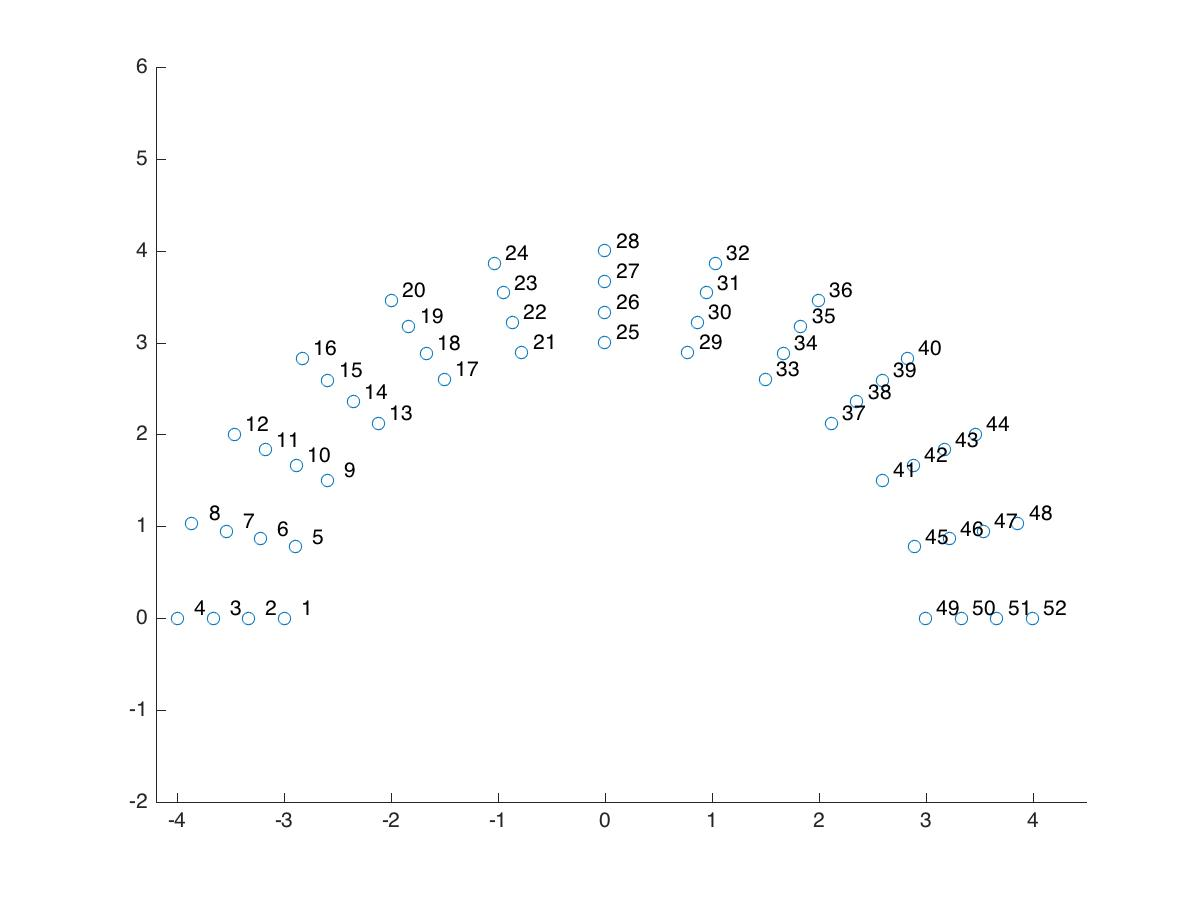
\includegraphics[width=10cm]{Mesh.jpg}
  \caption{Mesh for \(N_r=3, N_\theta=12\), with global node numbers given next to each node.}
  \label{fig:Mesh}
\end{figure}

\subsection{The Connectivity Matrix}

In order for this mesh to be useful for finite element implementation, a connectivity function must be defined to relate the local node numbering to the global node numbering. The connectivity matrix is an \(N\times4\) matrix, where \(N\) is the total number of elements and 4 is the number of local nodes per element (bilinear elements are assumed). The local node numbering is performed according to a counterclockwise fashion, beginning with the ``bottom left'' node of each element, as shown below:

\begin{equation}
\begin{aligned}
4 -- 3 \\
1 -- 2 \\
\end{aligned}
\end{equation}

The location matrix for the mesh shown in Fig. \ref{fig:Mesh} is shown below in order to illustrate the node numbering scheme and to be as explicit as possible about the meshing technique.

\begin{equation}
\textbf{LM}=
\begin{bmatrix}
1 & 5 & 6 & 2 \\
2 & 6 & 7 & 3 \\
3 & 7 & 8 & 4 \\
5 & 9 & 10 & 6 \\
6 & 10 & 11 & 7 \\
7 & 11 & 12 & 8 \\
9 & 13 & 14 & 10 \\
10 & 14 & 15 & 11 \\
11 & 15 & 16 & 12 \\
13 & 17 & 18 & 14 \\
14 & 18 & 19 & 15 \\
15 & 19 & 20 & 16 \\
17 & 21 & 22 & 18 \\
18 & 22 & 23 & 19 \\
19 & 23 & 24 & 20 \\
21 & 25 & 26 & 22 \\
22 & 26 & 27 & 23 \\
23 & 27 & 28 & 24 \\
25 & 29 & 30 & 26 \\
26 & 30 & 31 & 27 \\
27 & 31 & 32 & 28 \\
29 & 33 & 34 & 30 \\
30 & 34 & 35 & 31 \\
31 & 35 & 36 & 32 \\
33 & 37 & 38 & 34 \\
34 & 38 & 39 & 35 \\
35 & 39 & 40 & 36 \\
37 & 41 & 42 & 38 \\
38 & 42 & 43 & 39 \\
39 & 43 & 44 & 40 \\
41 & 45 & 46 & 42 \\
42 & 46 & 47 & 43 \\
43 & 47 & 48 & 44 \\
45 & 49 & 50 & 46 \\
46 & 50 & 51 & 47 \\
47 & 51 & 52 & 48 \\
\end{bmatrix}
\end{equation}

\section{Appendix}

This section contains the complete code used in this assignment. 
\begin{comment}
\subsection{\texttt{MeshGenerator.m}}
This program generates the mesh and connectivity matrix.
\lstinputlisting[language=Matlab]{MeshGenerator.m}
\end{comment}

\end{document}